\subsection{Methodology}
\subsubsection{Data Collection}
In the beginning our idea was to automate the data collection by using OpenWPM, a tool that automates the tasks of controlling a browser and collecting data. However, after some time it turned out that the general effort to set up such automation is not proportionate to the data we ultimately need. The only advantage would have been to replicate the user journey one-to-one and then possibly have more consistent data available. Nevertheless, we are now continuing with the manual data collection approach.

To analyze the cross-device tracking capabilities of various news websites, we conducted a systematic data collection using HTTP Archive (HAR) files. This process involved capturing network traffic data from both desktop and mobile devices. We selected our set of 20 websites by first categorizing them into news websites and shopping websites. These websites were chosen based on their popularity and the diversity of their content and geographical origin.

Prior to data collection, we created a test account on each of the selected websites. This was essential to ensure consistency in the user experience and to capture potential deterministic cross device tracking data across different sessions and devices.

To standardize the browsing environment and eliminate the most external variables, the data collection was executed using a virtual machine. This enables us to attribute any differences observed in the tracking mechanisms to the device type rather than other environmental factors.

Google Chrome was used as the web browser for this exercise as its developer tools with many functionalities allowed us to generate the HAR files. 

The first part of the data collection involved accessing each news website from a desktop device. The user journey for all websites of both categories started with logging in using the previously created test account. For news websites the second part was navigating to a prominent news topic and try to imitate common user behavior. For shopping websites the second part included adding one or more items to the shopping cart and then proceed to checkout, but stop just before the actual payment. 

The same procedure was replicated on mobile devices, to be more precise on an iPhone, in order capture the mobile user experience on the same websites. The HAR files of the mobile user journey was captured using Safari Developer Tools while connecting the iPhone to the MacBook via cable.

The resulting data set comprised 40 HAR files - 10 from desktop devices and 10 from mobile devices, corresponding to the same set of news websites and shopping websites. This data set will be the starting point for our subsequent analysis of cross-device tracking practices.
\subsubsection{Data Analysis}

\begin{figure}[ht]
    \centering
    \begin{subtable}[b]{0.3\textwidth}
        \centering
        \begin{tabular}{|l|l|}
            \hline
            \multicolumn{2}{|c|}{\textbf{cookieLog}} \\
            \hline
            id           & INT \\
            domain       & TEXT \\
            host         & TEXT \\
            device\_type  & TEXT \\
            website\_type & TEXT \\
            \hline
        \end{tabular}
        \caption{cookieLog}
    \end{subtable}
    \hfill
    % Table 2: emailHashes
    \begin{subtable}[b]{0.3\textwidth}
        \centering
        \begin{tabular}{|l|l|}
            \hline
            \multicolumn{2}{|c|}{\textbf{emailHashes}} \\
            \hline
            id           & INT \\
            host         & TEXT \\
            hash\_type    & TEXT \\
            domain       & TEXT \\
            device\_type  & TEXT \\
            website\_type & TEXT \\
            \hline
        \end{tabular}
        \caption{emailHashes}
    \end{subtable}
    \hfill
    \begin{subtable}[b]{0.3\textwidth}
        \centering
        \begin{tabular}{|l|l|}
            \hline
            \multicolumn{2}{|c|}{\textbf{thirdPartyLog}} \\
            \hline
            id           & INT \\
            domain       & TEXT \\
            host         & TEXT \\
            device\_type  & TEXT \\
            website\_type & TEXT \\
            \hline
        \end{tabular}
        \caption{thirdPartyLog}
    \end{subtable}
\end{figure}
Since our data is relatively large (50-100MB per HTTP archive), we performed most of the analysis using Jupyter Notebooks and the Python library haralyzer. In the initial stages of our data analysis, we began with a traditional approach, using print statements to inspect and debug the data. This method, while straightforward, quickly proved to be inadequate for handling larger datasets. As the volume and complexity of the data increased, it became apparent that a more robust and scalable solution was necessary. We then started to set up a database that includes three tables as displayed above, so we can perform the major part of our analysis with a small delay using simple SQL statements.

Our approach was then to determine which parts of the HTTP requests are relevant for us to make statements about cross-device tracking activities.

The first and perhaps most important part of our analysis consisted of filtering out HTTP requests that were sent to third-party domains. We are particularly interested in which domain the request was sent to and how often requests to such domains were recorded. We also wanted to compare the websites with each other in terms of the number of requests to third-party providers. We used the thirdPartyLog table in our database to filter and visualize the respective requests.

It is also interesting to see whether any sensitive data was sent to third-party providers. This means that we examine all HTTP requests and responses to see whether a simple, hashed or encrypted version of our email address can be found. We looked for plain and base64 encoded versions of our mail address as well as SHA1, SHA256, SHA224 and SHA512. In order filter and visualize our results, we used the emailHashes table of our database.

To get a general overview of the cookies set, we also wanted to determine the specific domains that have set the most cookies and possibly establish a correlation with the third-party domains that were requested the most. We focused on the quantity of cookies set by each domain, offering insight into the role these entities play in the broader context of online tracking, particularly in cross-device scenarios. We used the cookieLog table for this part.

In order to also qualitatively analyze the cookies that were set, we looked at each website to see if there were identical cookies that were set for the same website on the desktop and the mobile device. To be even more specific, we checked which cookies could be identifiers that are used to uniquely identify a user across multiple devices so that, for example, customized advertising can be placed. This part is done manually as we have to look at possible identifiers by ourselves, because it is difficult to automatically filter out identifiers.

In the last part of our analysis, we wanted to carry out a comparative analysis. In fact, we have two variables that seem interesting for comparison. First, the device type, to show differences in behavior between mobile and desktop devices, and second, the website category by which we divided our websites in the initial step.

Our plan was to conduct the previous analysis again, but this time to differentiate and look at the relevant category. In the best case scenario, we can see interesting results that give an indication of which categories are more affected by cross device tracking activities.

\subsection{Results}
\subsubsection{Requests to third party domains}
\subsubsection{Requests to third party domains}
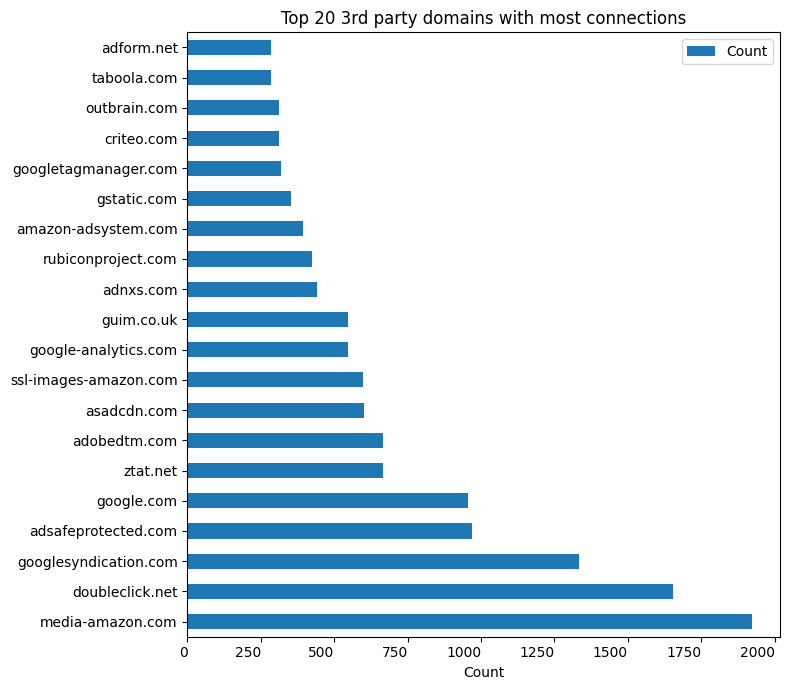
\includegraphics[width=0.95\textwidth]{./assets/top20thirdpartydomains.png}

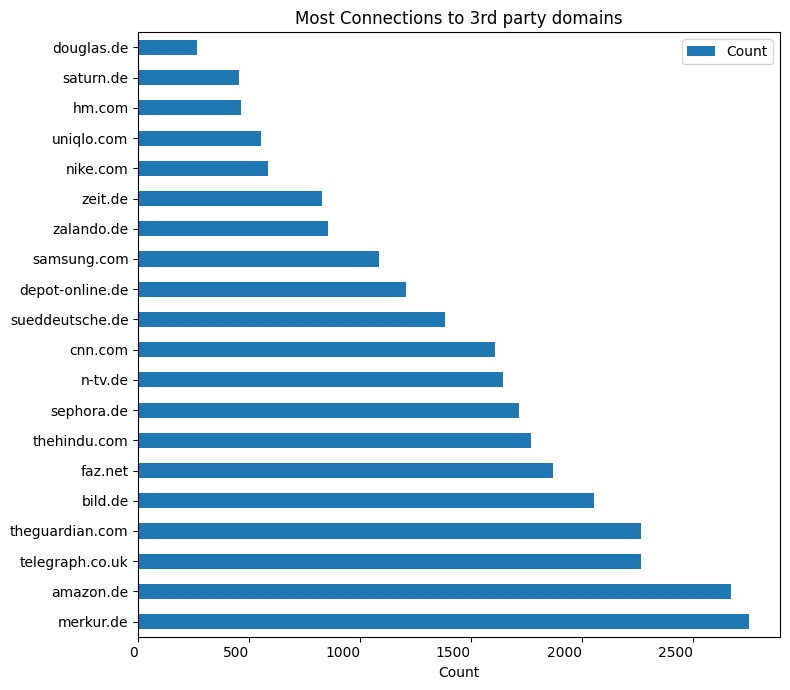
\includegraphics[width=0.95\textwidth]{./assets/mostConnectionsToThirdPartyDomains.png}

\subsubsection{Sensitive Information to third party providers}
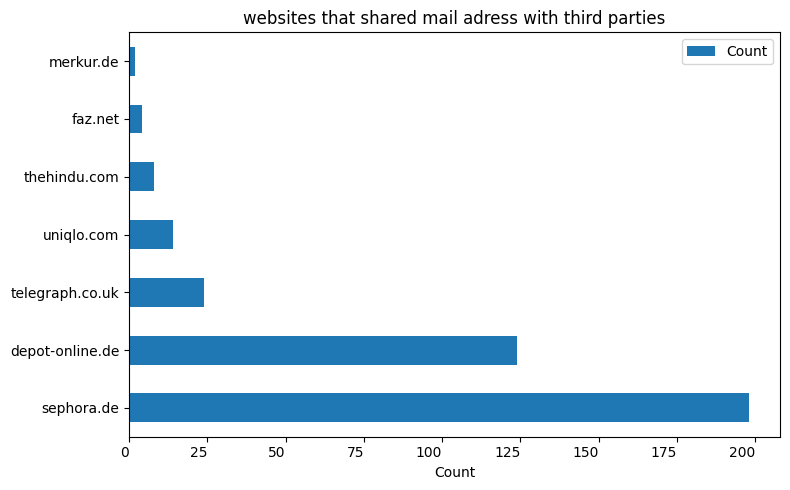
\includegraphics[width=0.95\textwidth]{./assets/websitesSharingMailAddresses.png}

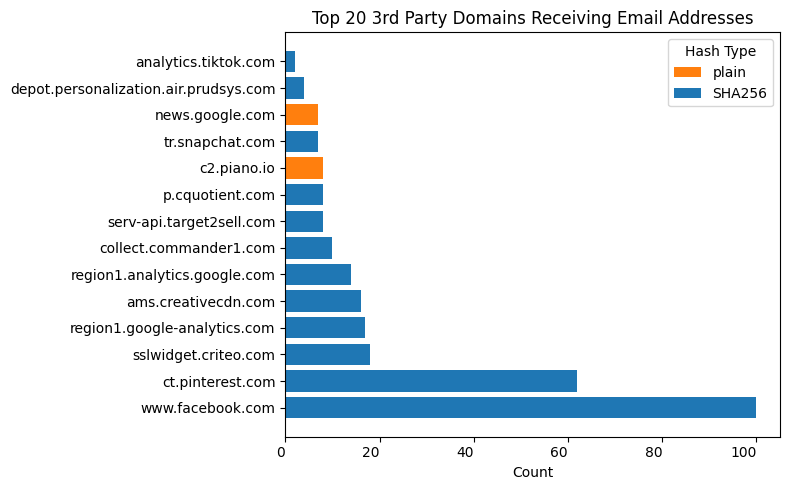
\includegraphics[width=0.95\textwidth]{./assets/top20thirdpartydomainsreceivingmailaddresses.png}

\subsubsection{Cookie Analysis}
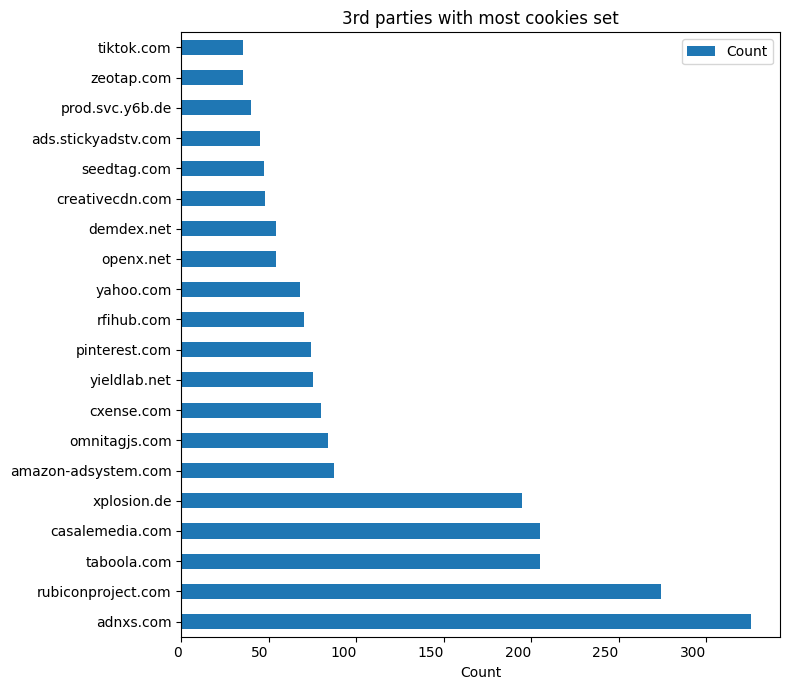
\includegraphics[width=0.95\textwidth]{./assets/thirdpartieswithmostcookiesset.png}

\subsubsection{Duplicate identifiers across mibile and desktop devices}